\documentclass[11pt,letterpaper]{article}
\usepackage[lmargin=1in,rmargin=1in,tmargin=1in,bmargin=1in]{geometry}
\usepackage{../style/homework}
\usepackage{../style/commands}
\setbool{quotetype}{true} % True: Side; False: Under
\setbool{hideans}{true} % Student: True; Instructor: False

% -------------------
% Content
% -------------------
\begin{document}

\homework{8: Due 03/29}{You only live once, but if you do it right, once is enough.}{Mae West}

% Problem 1
\problem{10} Give a rough sketch of the quadratic function $y= 8 - (x + 7/2)^2$. Your sketch should include the vertex and axis of symmetry. 
	\[
	\fbox{
	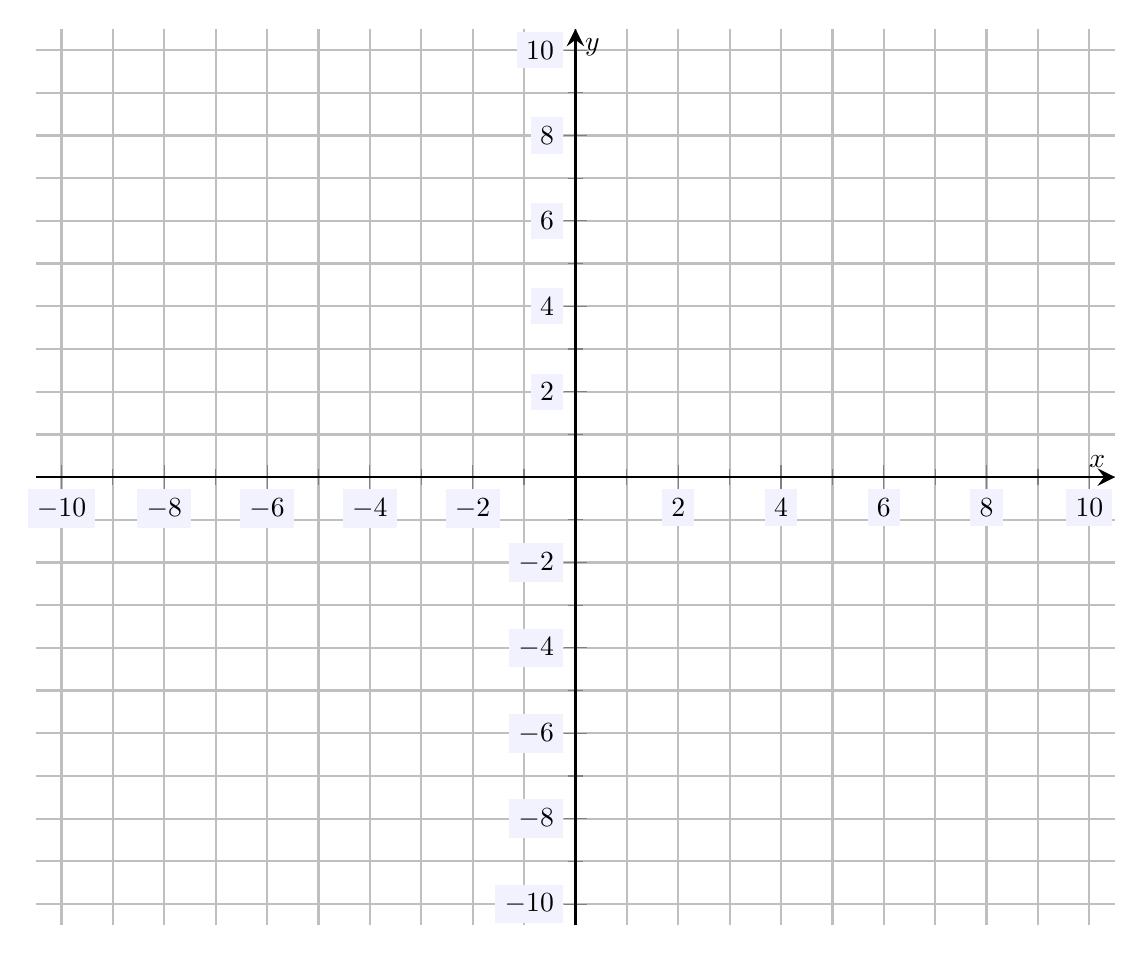
\begin{tikzpicture}[scale=2,every node/.style={scale=0.5}]
	\begin{axis}[
	grid=both,
	axis lines=middle,
	ticklabel style={fill=blue!5!white},
	xmin= -10.5, xmax=10.5,
	ymin= -10.5, ymax=10.5,
	xtick={-10,-8,-6,-4,-2,0,2,4,6,8,10},
	ytick={-10,-8,-6,-4,-2,0,2,4,6,8,10},
	minor tick = {-10,-9,...,10},
	xlabel=\(x\),ylabel=\(y\),
	]
	\end{axis}
	\end{tikzpicture}
	}
	\]



\newpage



% Problem 2
\problem{10} Find the vertex form of the function $f(x)= 8x^2 + 24x + 13$ both by completing the square and using the `evaluation-method.'



\newpage



% Problem 3
\problem{10} Consider the function $f(x)= (x - 8)^2 - 27$. 
	\begin{enumerate}[(a)]
	\item Determine if the given parabola opens upwards or downwards.
	\item Is the parabola convex or concave?
	\item Does the function $f(x)$ have a maximum or a minimum?
	\item Find the vertex and axis of symmetry. 
	\item Find the maximum/minimum value of $f(x)$. 
	\end{enumerate}



\newpage



% Problem 4
\problem{10} Consider the function $f(x)= x^2 + 6x + 3$. 
	\begin{enumerate}[(a)]
	\item Find the vertex form of $f(x)$. 
	\item Determine if the given parabola opens upwards or downwards.
	\item Is the parabola convex or concave?
	\item Does the function $f(x)$ have a maximum or a minimum? Find this value.
	\item Find the vertex and axis of symmetry. 
	\end{enumerate}


\end{document}